\documentclass[11pt,fleqn]{article}

\setlength {\topmargin} {-.15in}
\setlength {\textheight} {8.6in}

\usepackage{amsmath}
\usepackage{amssymb}
\usepackage{color}
\usepackage{tikz}
\usetikzlibrary{automata,positioning,arrows}
\usepackage{diagbox}



\newcommand{\be}{\begin{enumerate}}
\newcommand{\ee}{\end{enumerate}}

\begin{document}
\textbf{Exercise 5.4.4 NFA Drawing} Draw the NFA corresponding to the pattern $(((A|B)*|CD*|EFG)*)*$\\

\textbf{Solution:}

\begin{center}
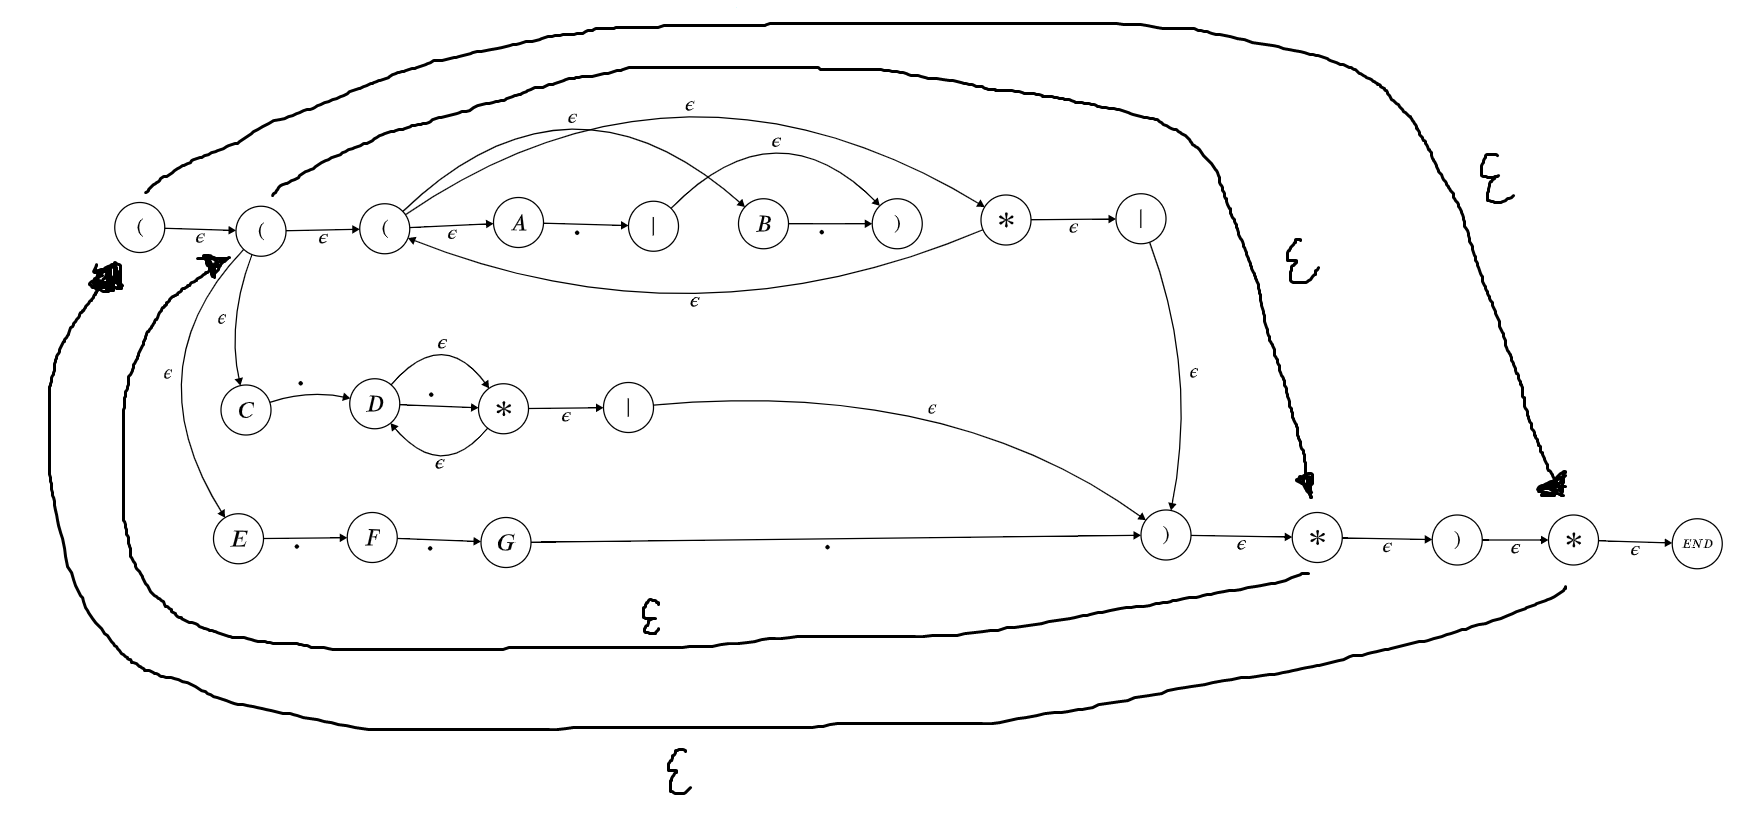
\includegraphics[scale=.7]{5.4.4.png}
\end{center}

\end{document}
